\section{判据用于 GFM 变流器时的局限}
\label{sec:lim}

本节说明定理~\ref{thm:dec_mixed_small_gain_phase} 的稳定性条件为何难以在实际电力系统应用中满足。构网型（GFM）变流器是一个典型例子，因为它通常具有很高的低频增益。为展示这一限制，我们考虑一台采用虚拟同步机（VSM）功率控制的常规 GFM 变流器（详见附录~\ref{apx:GFM_control}），通过短路比较低（SCR 低，即电网阻抗较大）的网络接入无限大母线，见图~\ref{fig:gfm_diag}。所得反馈环路的小增益和小相位曲线如图~\ref{fig:GFM_gain_phase_test} 所示。

该例揭示了三个主要问题：
\begin{itemize}
\item \textbf{违反小增益条件：}变流器增益显著超过电网增益，因此小增益条件始终不能满足。
\item \textbf{违反扇形性：}在 $0.9$ Hz 以下，变流器导纳不具有扇形性，因而不能应用小相位判据。
\item \textbf{保守性：}即使导纳具有扇形性且相位定义良好，在 $50$ Hz 以下，变流器与电网的相位区间也非常接近重叠，并最终在约 $1$ Hz 处发生重叠。这种重叠并不一定意味着系统实际不稳定，而可能只是小相位判据保守性的结果。
\end{itemize}
由此可见，经典小增益与小相位判据在现实的变流器主导场景中存在显著局限。下文进一步分析这种非扇形性的来源。

\begin{figure}[tbh]
\centering
\begin{subfigure}{\columnwidth}
  \centering
  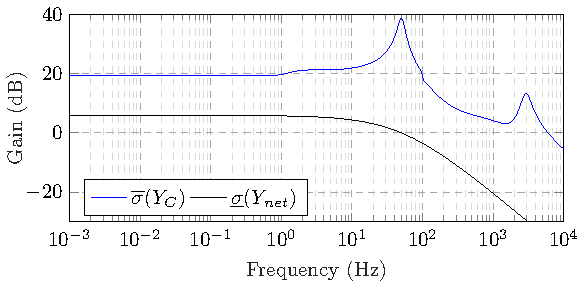
\includegraphics[width=\linewidth]{Gain_adm.pdf}
\end{subfigure}
\begin{subfigure}{\columnwidth}
  \centering
  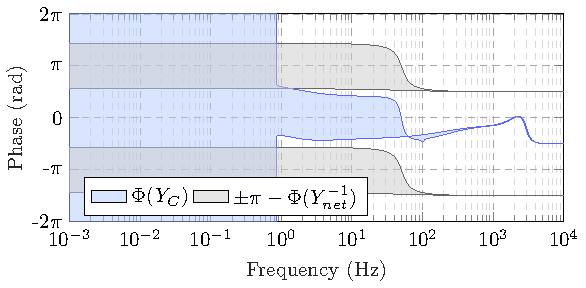
\includegraphics[width=\linewidth]{Phase_adm.pdf}
\end{subfigure}
\caption{GFM 变流器的混合小增益--相位条件。若系统不具有扇形性，则以完整区间 $[-2\pi,2\pi]$ 表示其相位。变流器增益超过网络增益时，小增益条件被违反；变流器相位与平移 $\pm\pi$ 后的网络相位重叠时，小相位条件被违反。}
\label{fig:GFM_gain_phase_test}
\end{figure}

\subsection{GFM 变流器的非扇形性}
如上例及其他研究所示，变流器导纳在低频段经常不具有扇形性~\cite{huangGainPhaseDecentralized2024,woolcockMixedGainPhase2023}。然而，这一现象的来源尚未得到充分研究：它究竟是特定控制架构与参数选择造成的，还是设备本身的固有属性，仍不清楚。

本文采用文献~\cite{guImpedanceBasedWholeSystemModeling2021} 的建模方法。一般变流器的小信号导纳模型如图~\ref{fig:frame_embedding} 所示。模型输入为局部稳态 $DQ$ 坐标系下公共耦合点电压 $V_{DQ}$，输出为同一坐标系下的变流器电流 $I_{DQ}$。变流器控制器工作在局部摆动 $dq$ 坐标系中，在概念上分为两部分：
\begin{itemize}
\item 同步控制器 $K_v(s)$，产生用于将变量从局部稳态坐标系变换到摆动坐标系的角度 $\epsilon$；
\item 其余控制系统 $Y_{dq}(s)$，包括电流控制、电压控制、虚拟阻抗、无功功率控制以及其他与同步无关的控制器。
\end{itemize}
局部稳态坐标系下的闭环导纳可写为
\begin{equation}
Y_{DQ}(s)=(Y_{dq}(s)+I_0^eK_v(s))(I+V_0^eK_v(s))^{-1}.
\label{eq:frame_embedding}
\end{equation}
其中，向量 $V_0^e=[-V_{q,0},V_{d,0}]^T$ 和 $I_0^e=[-I_{q,0},I_{d,0}]^T$ 表示两个坐标系之间旋转关系的线性化项；$V_{d,0},V_{q,0},I_{d,0},I_{q,0}$ 为电压和电流运行点。

\begin{figure}
\centering
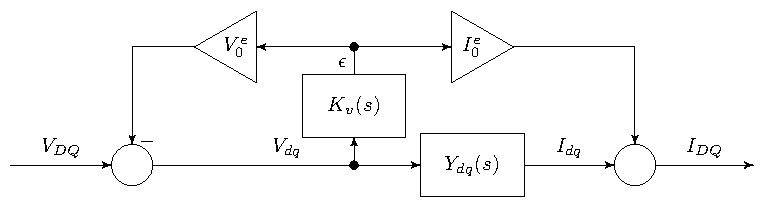
\includegraphics[width=\linewidth]{frame_embedding.pdf}
\caption{嵌入同步坐标系的一般变流器小信号模型。}
\label{fig:frame_embedding}
\end{figure}

对于采用功率同步的典型 GFM 变流器，角度 $\epsilon$ 由式~\eqref{eq:freq_tf} 所示动态系统产生，其中 $\omega$ 为频率，$P$ 为有功功率，$H_P(s)$ 为基于功率的同步环节传递函数：
\begin{equation}
\omega=H_P(s)P,\qquad \epsilon=\frac{1}{s}\omega.
\label{eq:freq_tf}
\end{equation}
对功率表达式线性化得到式~\eqref{eq:power_lin}。其中 $P$ 仅依赖局部稳态坐标系下的电压，因此 $K_v(s)$ 可写成式~\eqref{eq:Kv}：
\begin{equation}
P\approx\underbrace{(V_0Y_{dq}+I_0)}_{:=G_P(s)}V_{dq},\quad
V_0=[V_{d,0}\ V_{q,0}],\quad I_0=[I_{d,0}\ I_{q,0}],
\label{eq:power_lin}
\end{equation}
\begin{equation}
K_v(s)=\frac{H_P(s)}{s}G_P(s).
\label{eq:Kv}
\end{equation}

由于本文关注低频行为，下面考察 $s=j0$ 时的导纳直流增益。关键结果概括如下。

\begin{prop}
假设 $V_{q,0}=0$、$V_{d,0}\neq0$，且 $K_v(s)V_0^e$ 不恒为零。将式~\eqref{eq:Kv} 的 $K_v(s)$ 代入式~\eqref{eq:frame_embedding}，则变流器导纳矩阵在 $s=0$ 时为
\begin{equation}
Y_{DQ}(0)=
\begin{bmatrix}
-\dfrac{I_{d,0}}{V_{d,0}} & -\dfrac{I_{q,0}}{V_{d,0}}\\
\beta & \dfrac{I_{d,0}}{V_{d,0}}
\end{bmatrix},
\label{eq:Y_DQ_0}
\end{equation}
其中 $\beta$ 为某个标量。此外，$Y_{DQ}(0)$ 不具有扇形性。
\label{prop:Y_DQ_0}
\end{prop}

\begin{proof}
式~\eqref{eq:Y_DQ_0} 的推导见附录~\ref{apx:Prop_Y_DQ_0}。由于矩阵迹为零，特征值之和也为零。$2\times2$ 矩阵的数值域是以两个特征值为焦点的椭圆。根据 $\beta$ 和 $I_{q,0}$ 的取值，其长轴为实轴或虚轴。两种情况下原点都属于数值域，因此该矩阵不是扇形矩阵。
\end{proof}

假设 $V_{q,0}=0$ 不失一般性，因为总能选择适当的旋转矩阵使其成立。此外，根据运行点和参数的不同，导纳可能不仅不是扇形矩阵，甚至不是拟扇形矩阵。该结果表明，无论具体控制如何实现，在 $0$ Hz 处都无法实现扇形性，并且在低频段通常也不能满足扇形性。根本原因是 GFM 变流器表现为恒功率负载/电源。即使实施频率下垂控制，使功率随频率变化，从导纳所描述的电压--电流关系看，变流器仍然是恒功率设备。

上述分析还表明，变流器在低频段不是无源的\footnote{此处“无源”采用电力电子文献中常见的宽松逐频率含义，即 $Y(j\omega)$ 的正实性。}。这一结论与文献~\cite{deyAnalysisPassivityCharacteristics2021} 一致，但适用范围更广，因为它不依赖特定的控制实现或参数值。

\begin{rem}
也可以对跟网型（GFL）变流器作类似分析。例如，采用同步旋转坐标系锁相环（SRF-PLL）时，$K_v(s)$ 的形式为 $\frac{H_{PLL}(s)}{s}[0,1]$。对于典型的基于 PI 的有功功率控制，所得导纳与式~\eqref{eq:Y_DQ_0} 具有相同形式。因此，关于低频非扇形性和缺乏无源性的结论同样适用于 GFL 变流器。
\end{rem}
